\title{Model}

{{navbar}}

\subsubsection{Model}

A probabilistic model is a joint distribution $p(\mathbf{x},
\mathbf{z})$ of data $\mathbf{x}$ and latent variables $\mathbf{z}$.
For more details, see the \href{/tutorials/model}{Probability Models tutorial}.

In Edward, we specify models using a simple language of random variables.
A random variable $\mathbf{x}$ is an object parameterized by
tensors $\theta^*$, where
the number of random variables in one object is determined by
the dimension of its parameters.

\begin{lstlisting}[language=Python]
from edward.models import Normal, Exponential

# univariate normal
Normal(mu=tf.constant(0.0), sigma=tf.constant(1.0))
# vector of 5 univariate normals
Normal(mu=tf.zeros(5), sigma=tf.ones(5))
# 2 x 3 matrix of Exponentials
Exponential(lam=tf.ones([2, 3]))
\end{lstlisting}

For multivariate distributions, the multivariate dimension is the
innermost (right-most) dimension of the parameters.

\begin{lstlisting}[language=Python]
from edward.models import Dirichlet, MultivariateNormalFull

# K-dimensional Dirichlet
Dirichlet(alpha=tf.constant([0.1] * K)
# vector of 5 K-dimensional multivariate normals
MultivariateNormalFull(mu=tf.zeros([5, K]), sigma=...)
# 2 x 5 matrix of K-dimensional multivariate normals
MultivariateNormalFull(mu=tf.zeros([2, 5, K]), sigma=...)
\end{lstlisting}

For a list of random variables supported in Edward, see the
\href{https://www.tensorflow.org/versions/master/api_docs/python/contrib.distributions.html}{TensorFlow distributions API}.
Edward random variables build on top of them.

Random variables are equipped with methods such as
\texttt{log_prob()}, $\log p(\mathbf{x}\mid\theta^*)$,
\texttt{mean()}, $\mathbb{E}_{p(\mathbf{x}\mid\theta^*)}[\mathbf{x}]$,
and \texttt{sample()}, $\mathbf{x}^*\sim p(\mathbf{x}\mid\theta^*)$.
Further, each random variable is associated to a tensor $\mathbf{x}^*$ in the
computational graph, which represents a single sample $\mathbf{x}^*\sim
p(\mathbf{x}\mid\theta^*)$.

% 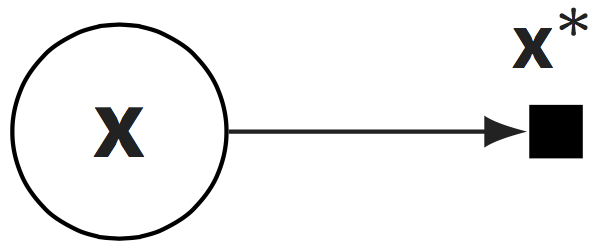
\includegraphics[width=225px]{/images/random_variable.png}

% This enables operations on the TensorFlow graph, allowing random
% variables to be used in conjunction with other TensorFlow ops.
This makes it easy to parameterize random variables with complex deterministic
structure, such as with deep neural networks and a diverse set of math
operations.
They operate on $\mathbf{x}^*$.

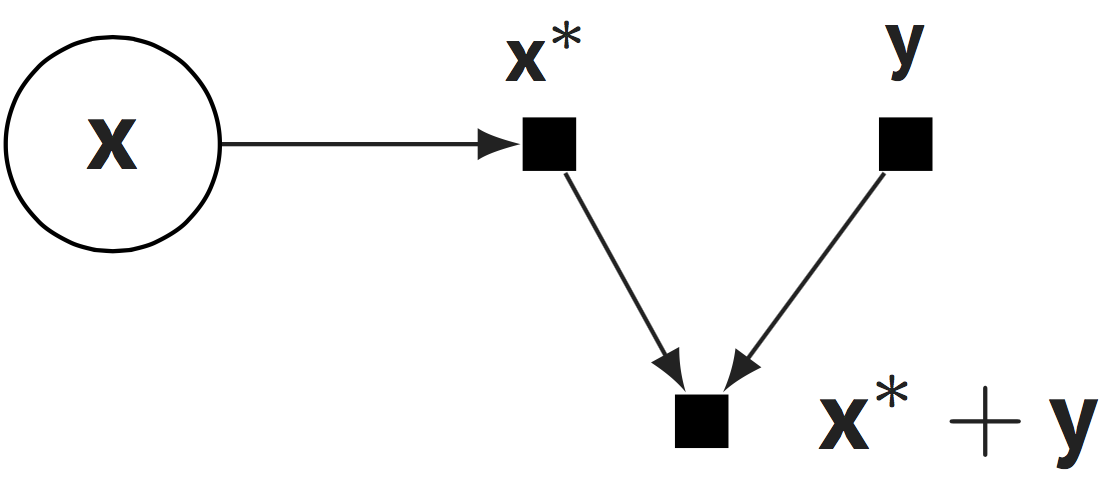
\includegraphics[width=375px]{/images/random_variable_ops.png}

\begin{lstlisting}[language=Python]
from edward.models import Normal

x = Normal(mu=tf.zeros(10), sigma=tf.ones(10))
y = tf.constant(5.0)
x + y, x - y, x * y, x / y
tf.tanh(x * y)
tf.gather(x, 2)  # 3rd normal rv in the vector
\end{lstlisting}

The design also enables compositions of random variables
to capture complex stochastic structure.
%
Below we illustrate a Beta-Bernoulli model,
\begin{equation*}
p(\mathbf{x}, \theta) =
\text{Beta}(\theta\mid 1, 1)
\prod_{n=1}^{50} \text{Bernoulli}(x_n\mid \theta),
\end{equation*}
where $\theta$
is a latent probability shared across the 50 data points $\mathbf{x}\in\{0,1\}^{50}$.

\begin{lstlisting}[language=python]
from edward.models import Bernoulli, Beta

theta = Beta(a=1.0, b=1.0)
x = Bernoulli(p=tf.ones(50) * theta)
\end{lstlisting}

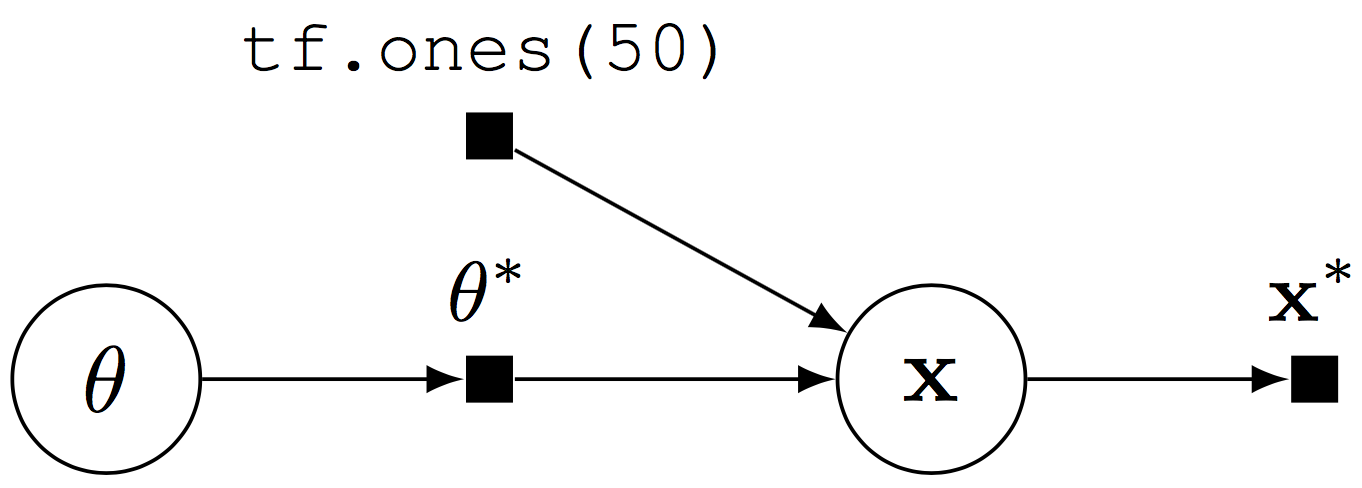
\includegraphics[width=450px]{/images/beta_bernoulli.png} \\
{\small\textit{%
Computational graph for a Beta-Bernoulli program.
}}

The random variable $\mathbf{x}$ is 50-dimensional, parameterized by the
random tensor $\theta^*$. Fetching the object $\mathbf{x}$ runs the
graph: it simulates from the generative process and
outputs a binary vector of $50$ elements.

With computational graphs, it is also natural to build mutable states
within the probabilistic program. As a typical use of computational
graphs, such states can define model parameters, that is, parameters
that we will always compute point estimates for and not be uncertain
about. In TensorFlow, this
is given by a \texttt{tf.Variable}. Another use case is for building
discriminative models $p(\mathbf{y}\mid\mathbf{x})$, where
$\mathbf{x}$ are features that are input as training or test data.  The
program can be written independent of the data, using a mutable state
(\texttt{tf.placeholder}) for $\mathbf{x}$ in its graph.
During training and testing, we feed the placeholder the appropriate
values.

For examples of models built in Edward, see the model
\href{/tutorials/}{tutorials}.
